%%%
%%% OpenCAEシンポジウムTeXテンプレートファイル
%%% template_OpenCAE_symposium.tex
%%% OpenCAEシンポジウム2018版
%%%
%%
%% ltjocはOpenCAE論文集・シンポジウム用のクラスファイルです.変更しないでください.
%% 本文が英語の場合には,オプションにenglishを指定してください.
\documentclass{../../style/ltjoc}
%\documentclass[english]{../../style/ltjoc}
%%
%% 表題(title),副題(subtitle),著者(author),所属(affiliation)
%% 本文が英語の場合には,こちらに英文表題,英文副題,英文著者,英文所属を記述します.
\title{GetFEM++ ユーザドキュメントの地域化L10N}
% 副題が無い場合にはコメントアウトします.
\subtitle{日本語翻訳作業} 
\author{%
\href{https://twitter.com/tkoyama010}{@tkoyama010}$^{1\dagger}$%
}
\affiliation{%
${}^{1}$\href{https://tkoyama010.github.io/getfem-docs-html-ja/}{GetFEM++ 日本語チーム}%
} 
%%
%% Corresponding authorの電子メールアドレス
%% 本論文について連絡が取れる著者の電子メールアドレスを記載してください.
\AuthorsEmail{tkoyama010@gmail.com}
%%
%% 英文表題(etitle),英文副題(esubtitle),英文著者(eauthor),英文所属(eaffiliation)
%% 本文が英語の場合には表示されません.
\etitle{Localization(L10N) of GetFEM++ User Document}
% 副題が無い場合にはコメントアウトします.
\esubtitle{Translation for Japanese}
\eauthor{%
\href{https://twitter.com/tkoyama010}{@tkoyama010}$^{*\dagger}$%
}
\eaffiliation{%
${}^{*}$\href{https://tkoyama010.github.io/getfem-docs-html-ja/}{GetFEM++ Japanese Team}%
}
%%
%% キーワード
\keywords{GetFEM++, L10N, SPHINX, Transifex, translate-shell}
%%
%% 英文概要
%% 英文概要を省略する場合には,abstract環境の定義をしないでください.
\begin{abstract}
The GetFEM++ project focuses on the development of a generic and efficient C++ library for finite element methods elementary computations.
The document of this library are generated by SPHINX and are available for modification and reuse under the terms of the GNU FDL().
\end{abstract}
%%
%% luatexja-fontspecパッケージ
\usepackage{luatexja-fontspec}
\defaultfontfeatures{Ligatures=TeX}
%% luatexja-presetパッケージ
%% 和文フォントのプリセット設定
%% オプションにnoembed(非埋込)を指定しないでください.
%\usepackage[ipaex]{luatexja-preset} % IPAex(デフォルト)
%\usepackage[ms]{luatexja-preset} % MS
%\usepackage[hiragino-pro]{luatexja-preset} % ヒラギノPro
%%
%% 欧文フォントの指定
%% 使用できるフォントについては,以下のコマンドで調べてください.
%% $ luaotfload-tool --list=*
%%
%% 欧文通常フォント
%\setmainfont{Cambria} % Cambria
%\setmainfont{Times New Roman} % Times New Roman
%\setmainfont{TeXGyreTermes} % TeXGyreTermes
%%
%% 欧文Sans-serifフォント
%\setsansfont{Calibri} % Calibri
%\setsansfont{Arial} % Arial
%\setsansfont{Helvetica} % Helvetica
%\setsansfont{TeXGyreHeros} % TeXGyreHeros
%%
%% 欧文monospaceフォント
%\setmonofont{Consolas} % Consolas
%\setmonofont{Courier New} % Courier New
%\setmonofont{Lucida Console} % Lucida Console
%%
%% subfigureパッケージ
\usepackage{subfigure}
%%
%% graphicxパッケージ
\usepackage{graphicx}
%%
%% shdocパッケージ
\usepackage[
 backgroundcolor=gray!50,
 usernamecolor=black,
 machinenamecolor=black,
 indicatorcolor=black,
 separatorcolor=black,
 pathcolor=black,
 optioncolor=black,
 textcolor=black
]{shdoc}
%%
%% underscoreパッケージ
\usepackage{underscore}
%%
%% draftwatermarkパッケージ
\usepackage{draftwatermark}
%%
%% hyperrefパッケージ
\usepackage[
 pdfencoding=auto,
 bookmarks=true,
 bookmarksnumbered=true,
 colorlinks=true,
 allcolors={blue}
]{hyperref}
%%
%% autorefでの図表の参照名の再定義
\makeatletter
\if@english
  \renewcommand*{\figureautorefname}{\figurename}
  \renewcommand*{\tableautorefname}{\tablename}
\else
  \renewcommand*{\figureautorefname}{図}
  \renewcommand*{\tableautorefname}{表}
\fi
\makeatother
%%
%% ヘッダ右の設定
%% シンポジウム毎に決められています.変更しないでください.
\markright{OpenCAE Symposium 2018, Dec. 8-9, 2018, Kawasaki} % Do not edit this line
%%
%% 本文
\begin{document}
%%
%% 題目などの出力
\maketitle
%%%
\section{はじめに}
GetFEM++は汎用的で効率的な有限要素法のC++ライブラリです。
ライブラリのドキュメントは、SPHINXで執筆されています。
また、\href{https://www.gnu.org/licenses/fdl.html}{GNU Free Documentation License}により改変および翻訳が許可されています。
そこで、本報告ではSPHINXの機能を使用したGetFEM++のドキュメント翻訳作業を紹介します。
さらに、技術同人誌即売会である\href{https://techbookfest.org/event/tbf05}{技術書典5}でドキュメントの頒布を行ったため、その様子についても報告します。
\section{\href{http://getfem.org}{GetFEM++}の説明}
まず、GetFEM++の全体像の把握のために、GetFEM++の英語のWikipediaを日本語に翻訳しました。
(\href{https://ja.wikipedia.org/wiki/Getfem++}{https://ja.wikipedia.org/wiki/Getfem++}を参照。)
以下に内容を引用します。
\section{\href{https://savannah.gnu.org}{GNU Savannah}の利用方法}
GetFEM++はソースのホスティングサービスとしてSavannahを使用しています。
GNU SavannahについてWikipediaの説明を引用します。
\begin{quote}
GNU Savannah は、フリーソフトウェアプロジェクトのための協働型ソフトウェア開発管理システムを提供するフリーソフトウェア財団のプロジェクトです。
現在は、CVS、GNU arch、Subversion、Git、Mercurial、GNU Bazaar、メーリングリスト、ウェブホスティング、ファイルホスティング、バグ管理サービスといった機能を提供しています。
Savannah は、SourceForge.netと同じソフトウェアをベースとしたホスティングサービスシステムである Savane を使っています。
(\texttt{Wikipediaより})
\end{quote}
このように、GNU SavannahはGNUプロジェクトやフリーソフトのホスティングサービスとして広く使われています。
非開発ユーザの場合、以下のようにして、リポジトリをクローンします。
\begin{shbox}
  \shuser{username}
  \shline{}{git clone https://git.savannah.nongnu.org/git/getfem.git}
\end{shbox}
また、ソースからコンパイルする必要のない場合には以下のように\texttt{aptitude}(もしくは\texttt{apt})コマンドによりインストールすることも可能です。
\begin{shbox}
  \shuser{username}
  \shline{}{sudo aptitude install python-getfem++ libgetfem++-dev}
\end{shbox}
これによりGetfem++のPythonインターフェースとライブラリがインストールされます。

一方、Savannahのプロジェクトの開発に参加するには\autoref{fig:savannah-new-user}の"New User"からユーザー登録が必要です。
%
\begin{figure}[htbp]
\centering
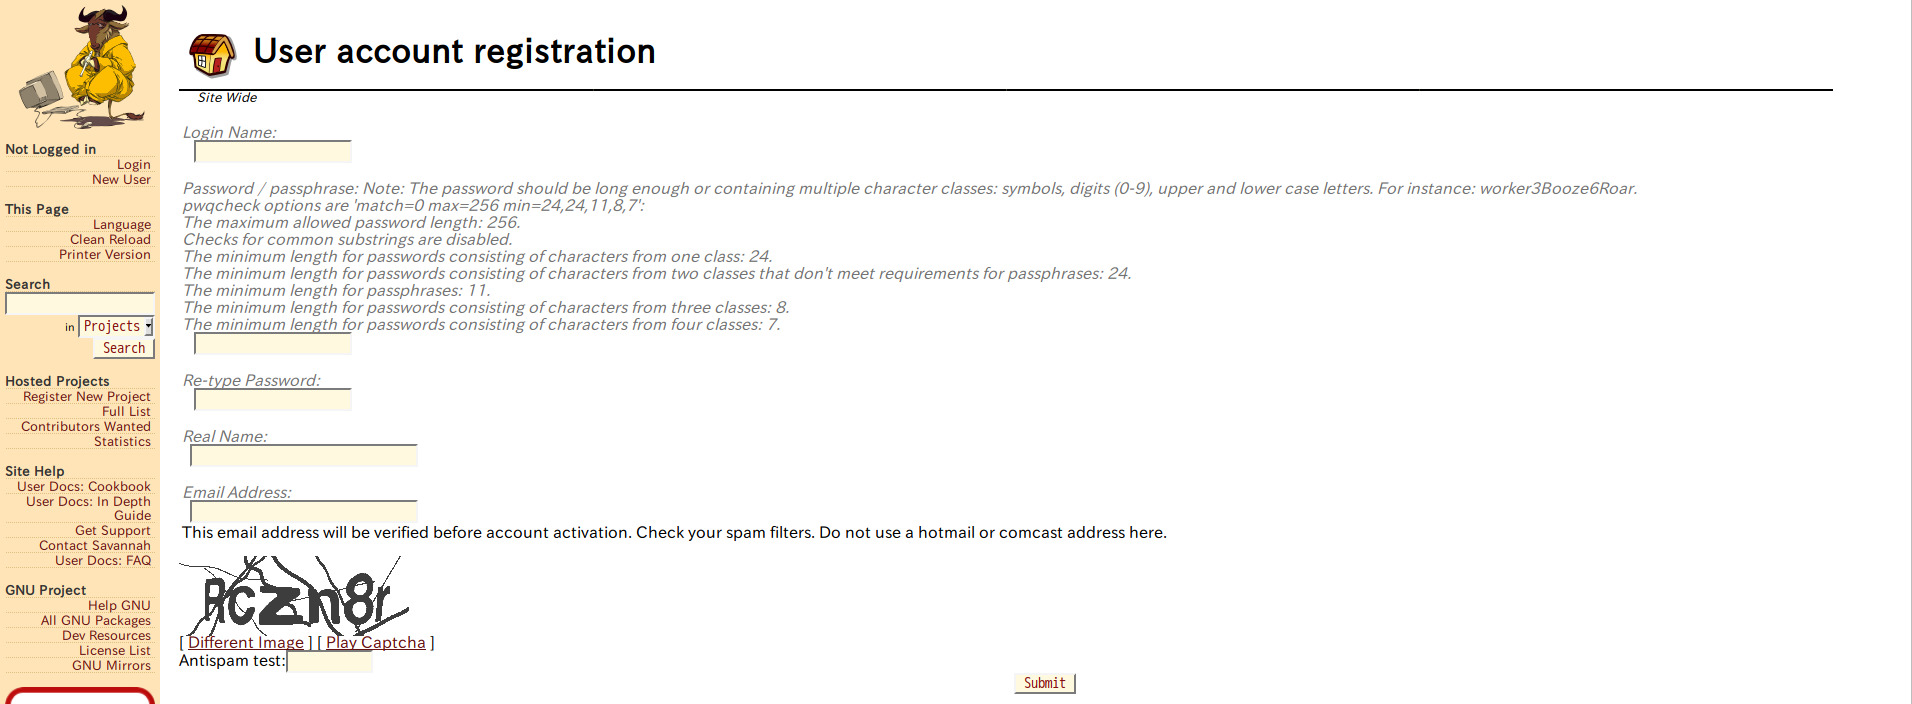
\includegraphics[width=1.0\textwidth]{fig/savannah-new-user.eps}
\caption{\href{https://savannah.gnu.org/account/register.php}{Savannahの新規ユーザ作成画面}}
\label{fig:savannah-new-user}
\end{figure}
開発者としてプロジェクトに参加するには、管理者にメッセージを送信し参加を承認してもらう必要があります。
2018年10月現在のGetFEM++の管理者は \href{http://www.dtu.dk/english/service/phonebook/person?id=65472&tab=2&qt=dtupublicationquery}{Konstantinos Poulios} 氏と \href{http://math.univ-lyon1.fr/~renard/}{Yves Renard} 氏です。
開発者として権限が与えられたら、\href{http://getfem.org/project/index.html}{How to contribute / Git repository on Savannah}を参考にプロジェクトにコミットをします。
開発者として、リポジトリをクローンする場合は以下のようにします。
\begin{shbox}
  \shuser{develname}
  \shline{}{git clone ssh://savannah-login@git.sv.gnu.org:/srv/git/getfem.git}
\end{shbox}
ここで、\texttt{savannah-login}はSavannahに登録したユーザ名です。
ただし、何の設定もせずこれを実行すると認証エラーが発生します。
このコマンドを実行する前にSavannahに認証鍵を登録しておく必要があります。
まずは、ホームディレクトリで\texttt{ssh-keygen}コマンドを実行して認証鍵を作成してください。
\begin{shbox}
  \shuser{develname}
  \shline{}{cd /home/develname}
  \shline{}{ssh-keygen}
  \shoutput{}{Generating public/private rsa key pair.}
  \shoutput{}{Enter file in which to save the key (/home/develname/.ssh/id\textunderscore{}rsa):}
  \shoutput{}{Created directory '/home/develname/.ssh'.}
  \shoutput{}{Enter passphrase (empty for no passphrase):}
  \shoutput{}{Enter same passphrase again:}
  \shoutput{}{Your identification has been saved in /home/develname/.ssh/id\textunderscore{}rsa.}
  \shoutput{}{Your public key has been saved in /home/develname/.ssh/id\textunderscore{}rsa.pub.}
  \shoutput{}{The key fingerprint is:}
  \shoutput{}{SHA256:NVKmqK8YvqZiSakm3NO5+zLkrlPARjZnmlDIvqKVWks develname@linux}
  \shoutput{}{以下略}
  \shline{}{}
\end{shbox}
これにより\texttt{/home/develname/.ssh/id\textunderscore{}rsa.pub}にRSA公開鍵のファイルが作成されます。
これを、Savannahに図YYYのように登録しておくと登録した認証鍵を持つPCに\texttt{clone}が可能になります。
\begin{figure}[htbp]
\centering
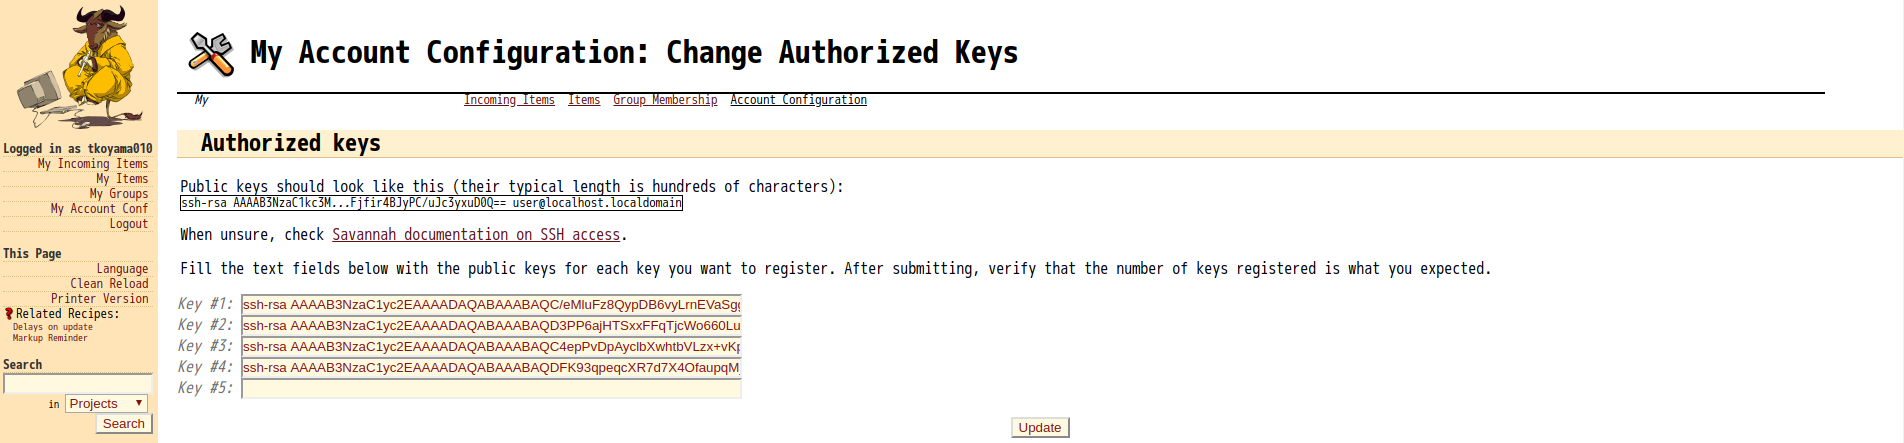
\includegraphics[width=1.0\textwidth]{fig/savannah-authorized-keys.eps}
\caption{\href{https://savannah.gnu.org/account/register.php}{Savannahの新規ユーザ作成画面}}
\label{fig:savannah-authorized-keys}
\end{figure}
変更を行う際にはGitで以下のようにブランチを作成する規約となっています。
\begin{shbox}
  \shuser{develname}
  \shline{}{cd /path/to/getfem}
  \shline{}{git branch devel-name-subject}
  \shline{}{git checkout devel-name-subject}
\end{shbox}
ここで、\texttt{name}は開発者の名前、\texttt{subject}は開発内容としてください。
\footnote{
プロジェクトへの貢献方法はプログラムの新機能のパッチ作成だけではありません。
ドキュメントを読んでいる際に気づいたTypo(打ち間違い)の修正も大切な貢献です。
筆者はTypoの修正のために\texttt{fixfixmisspell}という\texttt{branch}を作成したころ、Typo修正用の公式ブランチとして採用されました。
詳細は、 \href{http://getfem.org/project/contribute.html}{http://getfem.org/project/contribute.html} の"Specific branch for doc improvements and typo-fixes"を参照してください。
自分の小さな提案が採用されることもOSSへの貢献の面白さかと思います。
}
修正後コミットをしてブランチに\texttt{push}します。
\begin{shbox}
  \shuser{develname}
  \shline{}{cd /path/to/getfem}
  \shline{}{git commit -m"開発内容のメッセージ。もちろん英語!"}
  \shline{}{git push origin devel-name-subject}
\end{shbox}
修正後メーリングリスト\texttt{getfem-commits@nongnu.org}に連絡をして\texttt{master}ブランチへのマージを管理者にリクエストしてください。
\emph{誤って}\texttt{master}\emph{ブランチに}\texttt{push}\emph{しないように十分注意してください}!!!
管理者から注意されて\texttt{revert}されるでしょう。

\section{GetFEM++のコンパイル方法}
\texttt{Ubuntu18.04}でコンパイルする場合について説明します。
まずは、\texttt{getfem}のリポジトリ直下にある\texttt{autogen.sh}を実行します。
実行には\texttt{libtoolize}と\texttt{automake}が必要になりますので先にインストールしてください。
\begin{shbox}
  \shuser{devlname}
  \shline{} {sudo aptitude install libtool automake}
\end{shbox}
また、追加として以下のパッケージをインストールします。
\begin{itemize}
  \item \texttt{libopenblas-dev} - Optimized BLAS (linear algebra) library (development files)
%  \footnote{
%    \texttt{openblas}を使用すると通常の\texttt{blas}より高速になるとの指摘を\href{https://twitter.com/michioga}{@michioga}氏よりいただきました。
%    (第14回オープンCAE勉強会@関東(構造など))
%  }
\end{itemize}

\section{国際化L20Nと地域化L10N}
\section{\href{http://www.sphinx-doc.org/en/master}{SPHINX}の利用方法}
\section{\href{https://www.transifex.com}{Transifex}の利用方法}
\section{translate-shellの利用方法}
\section{GetFEM++の日本語キーワード}
\section{技術書典5の参加報告}
\section{まとめ}
\end{document}
